\documentclass[aspectratio=169]{beamer}
\usetheme{Madrid}
\usecolortheme{default}

\usepackage{tikz}
\usepackage{pgfplots}
\pgfplotsset{compat=1.18}
\usepackage{booktabs}
\usepackage{array}
\usepackage{colortbl}
\usepackage{xcolor}
\usepackage{fontawesome5}
\usepackage{amsmath}
\usepackage{amssymb}
\usetikzlibrary{shapes.geometric, arrows.meta, positioning, fit, backgrounds, calc, decorations.pathreplacing, shadows}

% ---- Color Palette ----
\definecolor{ddrblue}{RGB}{10, 40, 90}
\definecolor{ddracent}{RGB}{0, 153, 204}
\definecolor{ddrlite}{RGB}{220, 238, 255}
\definecolor{ddr2green}{RGB}{0, 130, 90}
\definecolor{ddr1orange}{RGB}{210, 100, 20}
\definecolor{lightgray2}{RGB}{240, 243, 248}
\definecolor{darktext}{RGB}{20, 20, 40}

% ---- Beamer Theme Overrides ----
\setbeamercolor{frametitle}{bg=ddrblue, fg=white}
\setbeamercolor{title}{fg=white}
\setbeamercolor{author}{fg=ddrlite}
\setbeamercolor{structure}{fg=ddrblue}
\setbeamercolor{block title}{bg=ddrblue, fg=white}
\setbeamercolor{block body}{bg=ddrlite}
\setbeamercolor{block title alerted}{bg=ddr1orange, fg=white}
\setbeamercolor{block body alerted}{bg=orange!10}
\setbeamercolor{block title example}{bg=ddr2green, fg=white}
\setbeamercolor{block body example}{bg=green!8}

\setbeamerfont{frametitle}{size=\large, series=\bfseries}
\setbeamerfont{title}{size=\LARGE, series=\bfseries}
\setbeamertemplate{navigation symbols}{}
\setbeamertemplate{footline}{%
  \leavevmode%
  \hbox{%
    \begin{beamercolorbox}[wd=.35\paperwidth,ht=2.4ex,dp=1ex,center]{frametitle}%
      \usebeamerfont{author in head/foot}\insertshortauthor
    \end{beamercolorbox}%
    \begin{beamercolorbox}[wd=.45\paperwidth,ht=2.4ex,dp=1ex,center]{frametitle}%
      \usebeamerfont{title in head/foot}\insertshorttitle
    \end{beamercolorbox}%
    \begin{beamercolorbox}[wd=.20\paperwidth,ht=2.4ex,dp=1ex,center]{frametitle}%
      \insertframenumber{} / \inserttotalframenumber
    \end{beamercolorbox}}%
}

% ---- TikZ Styles ----
\tikzset{
  block/.style={rectangle, rounded corners=3pt, draw=ddrblue, fill=ddrlite,
                text width=#1, align=center, minimum height=0.7cm, font=\small},
  block/.default=2.5cm,
  sblock/.style={rectangle, rounded corners=3pt, draw=ddrblue!60, fill=white,
                 text width=#1, align=center, minimum height=0.5cm, font=\scriptsize},
  sblock/.default=2.0cm,
  arrow/.style={-Stealth, thick, color=ddrblue},
  darrow/.style={Stealth-Stealth, thick, color=ddracent},
  ddr1box/.style={rectangle, rounded corners=4pt, draw=ddr1orange, fill=ddr1orange!12,
                  text width=#1, align=center, minimum height=0.6cm, font=\small\bfseries},
  ddr1box/.default=2.8cm,
  ddr2box/.style={rectangle, rounded corners=4pt, draw=ddr2green, fill=ddr2green!12,
                  text width=#1, align=center, minimum height=0.6cm, font=\small\bfseries},
  ddr2box/.default=2.8cm,
  highlight/.style={rectangle, rounded corners=2pt, draw=ddracent, fill=ddracent!15,
                    inner sep=3pt, font=\scriptsize},
}

\title[DDR1 \& DDR2 SDRAM]{DDR1 vs DDR2 SDRAM}
\subtitle{Memory Evolution and Technical Deep Dive}
\author[Technical Presentation]{Memory Architecture}
\date{}

\begin{document}

% ===================================================================
% SLIDE 1: TITLE
% ===================================================================
{
\setbeamercolor{background canvas}{bg=ddrblue}
\begin{frame}[plain]
  \vspace{2.0cm}
  \begin{center}
    {\color{white}\Huge\bfseries DDR1 vs DDR2 SDRAM}\\[0.5cm]
    {\color{ddrlite}\large Memory Architecture Evolution}\\[1.5cm]
    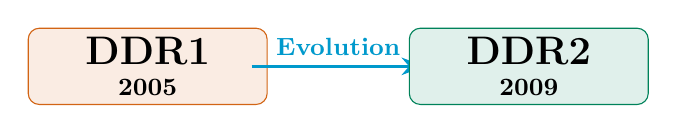
\begin{tikzpicture}[scale=1.1]
      \node[ddr1box=2.8cm, align=center] (d1) at (-2.2, 0) {{\Large DDR1}\\2005};
      \draw[-Stealth, very thick, ddracent] (-1.0, 0) -- (1.0, 0)
            node[midway, above, font=\small\bfseries, color=ddracent] {Evolution};
      \node[ddr2box=2.8cm, align=center] (d2) at (2.2, 0) {{\Large DDR2}\\2009};
    \end{tikzpicture}\\[0.8cm]
    {\color{ddrlite}\small JESD79 \& JESD79-2 Standards}
  \end{center}
\end{frame}
}

% ===================================================================
% SLIDE 2: MOTIVATION
% ===================================================================
\begin{frame}{Motivation: Why DDR Memory?}
  \begin{columns}[T]
    \begin{column}{0.50\textwidth}
      \textbf{SDR SDRAM Limitation:}
      \begin{itemize}
        \setlength\itemsep{8pt}
        \item Data valid on \textbf{rising edge only}
        \item 50\% bus utilization (falling edge wasted)
        \item Frequency scaling hit thermal/power limits
        \item Needed way to increase bandwidth without more MHz
      \end{itemize}
    \end{column}
    \begin{column}{0.48\textwidth}
      \vspace{0.3cm}
      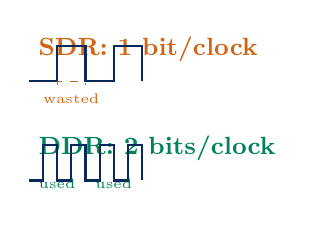
\begin{tikzpicture}[scale=0.9]
        % SDR
        \node[font=\small\bfseries, color=ddr1orange, anchor=west] at (0, 3.2) {SDR: 1 bit/clock};
        \draw[ddrblue, thick] (0, 3.0-0.25) -- (0.4, 3.0-0.25) -- (0.4, 3.0+0.25) -- (0.8, 3.0+0.25)
             -- (0.8, 3.0-0.25) -- (1.2, 3.0-0.25) -- (1.2, 3.0+0.25) -- (1.6, 3.0+0.25) -- (1.6, 3.0-0.25);
        \draw[ddr1orange, dashed, thin] (0.4, 2.7) -- (0.4, 3.0-0.25) -- (0.8, 3.0-0.25) -- (0.8, 2.7);
        \node[font=\tiny, color=ddr1orange] at (0.6, 2.5) {wasted};
        
        % DDR
        \node[font=\small\bfseries, color=ddr2green, anchor=west] at (0, 1.8) {DDR: 2 bits/clock};
        \draw[ddrblue, thick] (0, 1.6-0.25) -- (0.2, 1.6-0.25) -- (0.2, 1.6+0.25) -- (0.4, 1.6+0.25)
             -- (0.4, 1.6-0.25) -- (0.6, 1.6-0.25) -- (0.6, 1.6+0.25) -- (0.8, 1.6+0.25)
             -- (0.8, 1.6-0.25) -- (1.0, 1.6-0.25) -- (1.0, 1.6+0.25) -- (1.2, 1.6+0.25)
             -- (1.2, 1.6-0.25) -- (1.4, 1.6-0.25) -- (1.4, 1.6+0.25) -- (1.6, 1.6+0.25) -- (1.6, 1.6-0.25);
        \node[font=\tiny, color=ddr2green] at (0.4, 1.3) {used};
        \node[font=\tiny, color=ddr2green] at (1.2, 1.3) {used};
      \end{tikzpicture}
    \end{column}
  \end{columns}
  
  \vspace{0.5cm}
  \begin{exampleblock}{\small Solution: Capture on Both Clock Edges}
    Transfer data on rising \textbf{AND falling edges} of the same clock → doubles bandwidth without doubling frequency.
  \end{exampleblock}
\end{frame}

% ===================================================================
% SLIDE 3: DDR1 OVERVIEW
% ===================================================================
\begin{frame}{DDR1 (JESD79): Architecture Overview}
  \begin{columns}[T]
    \begin{column}{0.50\textwidth}
      \textbf{Key Features:}
      \begin{itemize}
        \setlength\itemsep{7pt}
        \item \textbf{2:1 Prefetch} → 2 bits per cell per access
        \item \textbf{4 Banks} with independent row buffers
        \item \textbf{VDD = 2.5 V}, SSTL\_2 I/O standard
        \item \textbf{DQS edge-aligned} to data (requires center logic)
        \item \textbf{No ODT} (external termination only)
      \end{itemize}
      \vspace{0.4cm}
      \begin{block}{\small Speed Grades}
        \footnotesize DDR-200 (10 ns), DDR-266 (7.5 ns), \\
        DDR-333 (6 ns), DDR-400 (5 ns)
      \end{block}
    \end{column}
    \begin{column}{0.48\textwidth}
      \vspace{0.2cm}
      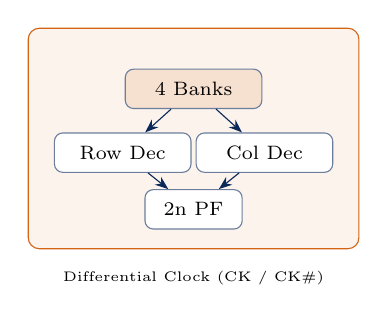
\begin{tikzpicture}[scale=0.9]
        \node[rectangle, rounded corners=4pt, draw=ddr1orange, fill=ddr1orange!8,
              minimum width=4.2cm, minimum height=2.8cm] (die) at (0,0) {};
        
        \node[sblock=1.5cm, fill=ddr1orange!20] (arr) at (0, 0.7) {4 Banks};
        \node[sblock=1.5cm] (row) at (-1.0, -0.2) {Row Dec};
        \node[sblock=1.5cm] (col) at (1.0, -0.2) {Col Dec};
        \node[sblock=1.0cm] (pf) at (0, -1.0) {2n PF};
        
        \draw[arrow, thin] (arr) -- (row);
        \draw[arrow, thin] (arr) -- (col);
        \draw[arrow, thin] (row) -- (pf);
        \draw[arrow, thin] (col) -- (pf);
        
        \node[font=\tiny, below=0.15cm of die.south] {Differential Clock (CK / CK\#)};
      \end{tikzpicture}
    \end{column}
  \end{columns}
\end{frame}

% ===================================================================
% SLIDE 4: DDR1 COMMAND FLOW
% ===================================================================
\begin{frame}{DDR1: Command Sequence (ACTIVATE → READ/WRITE → PRECHARGE)}
  \begin{columns}[T]
    \begin{column}{0.50\textwidth}
      \textbf{Read/Write Operation:}
      \vspace{0.2cm}
      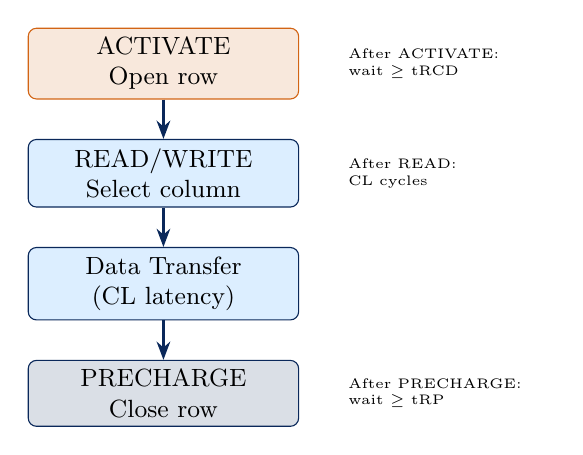
\begin{tikzpicture}[node distance=0.50cm]
        \node[block=3.2cm, fill=ddr1orange!15, draw=ddr1orange] (act) {ACTIVATE\\Open row};
        \node[block=3.2cm, below=of act] (read) {READ/WRITE\\Select column};
        \node[block=3.2cm, below=of read] (data) {Data Transfer\\(CL latency)};
        \node[block=3.2cm, below=of data, fill=ddrblue!15] (pre) {PRECHARGE\\Close row};
        
        \foreach \source/\target in {act/read, read/data, data/pre}
          \draw[arrow] (\source) -- (\target);
        
        % Constraints
        \node[font=\tiny, right=0.5cm of act, align=left, text width=2.5cm] (c1)
              {After ACTIVATE:\\ wait $\geq$ tRCD};
        \node[font=\tiny, right=0.5cm of read, align=left, text width=2.5cm] (c2)
              {After READ:\\ CL cycles};
        \node[font=\tiny, right=0.5cm of pre, align=left, text width=2.5cm] (c3)
              {After PRECHARGE:\\ wait $\geq$ tRP};
      \end{tikzpicture}
    \end{column}
    \begin{column}{0.48\textwidth}
      \vspace{0.2cm}
      \textbf{4-Bank Architecture:}
      \vspace{0.15cm}
      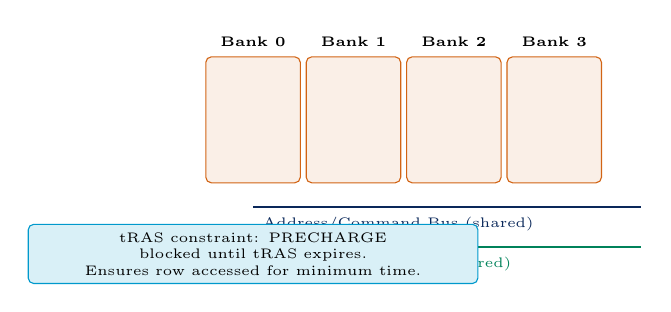
\begin{tikzpicture}[scale=0.85]
        % 4 banks
        \foreach \b/\pos in {0/0cm, 1/1.5cm, 2/3cm, 3/4.5cm} {
          \node[rectangle, draw=ddr1orange, fill=ddr1orange!10, minimum width=1.2cm,
                minimum height=1.6cm, rounded corners=2pt, label=above:{\tiny\bfseries Bank \b}] 
               at (\pos, 1.2) {};
        }
        
        % Shared buses
        \draw[ddrblue, thick] (0, -0.1) -- (5.8, -0.1);
        \node[font=\tiny, color=ddrblue, anchor=west] at (0, -0.35) {Address/Command Bus (shared)};
        
        \draw[ddr2green, thick] (0, -0.7) -- (5.8, -0.7);
        \node[font=\tiny, color=ddr2green, anchor=west] at (0, -0.95) {DQ Data Bus (64-bit, shared)};
        
        % Key constraint
        \node[highlight, below=0.3cm, text width=5.5cm, align=center, font=\tiny]
             {tRAS constraint: PRECHARGE blocked until tRAS expires.\\Ensures row accessed for minimum time.};
      \end{tikzpicture}
    \end{column}
  \end{columns}
\end{frame}

% ===================================================================
% SLIDE 5: DDR1 KEY TIMING
% ===================================================================
\begin{frame}{DDR1: Key Timing Parameters}
  \begin{columns}[T]
    \begin{column}{0.52\textwidth}
      \renewcommand{\arraystretch}{1.4}
      \begin{tabular}{>{\bfseries\small}l l}
        \toprule
        \textbf{Parameter} & \textbf{Typical (DDR-400)} \\
        \midrule
        \textcolor{ddr1orange}{CL} & 3 cycles (15 ns) \\
        \textcolor{ddr1orange}{tRCD} & 3 cycles (15 ns) \\
        \textcolor{ddr1orange}{tRP} & 3 cycles (15 ns) \\
        \textcolor{ddr1orange}{tRAS} & 8 cycles (40 ns) \\
        \textcolor{ddr1orange}{tWR} & 2 cycles \\
        tRFC & 12 cycles (72 ns) \\
        \bottomrule
      \end{tabular}
      \vspace{0.4cm}
      \begin{description}[\bfseries CL]
        \item[CL] Cycles from READ command to data valid
        \item[tRCD] Cycles from ACTIVATE to READ/WRITE
        \item[tRP] Cycles to fully close a row
        \item[tRAS] Min time row must stay open
      \end{description}
    \end{column}
    \begin{column}{0.46\textwidth}
      \vspace{0.1cm}
      \textbf{READ Timing (CL=3):}
      \vspace{0.2cm}
      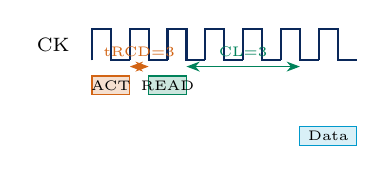
\begin{tikzpicture}[scale=0.8]
        \def\H{0.25} \def\T{0.6}
        
        % Clock
        \node[font=\scriptsize, anchor=east] at (-0.2, 2.6) {CK};
        \foreach \i in {0,1,2,3,4,5,6} {
          \pgfmathsetmacro\x{\i*\T}
          \draw[ddrblue, thick] (\x, 2.6-\H) -- (\x, 2.6+\H) -- (\x+\T/2, 2.6+\H)
               -- (\x+\T/2, 2.6-\H) -- (\x+\T, 2.6-\H);
        }
        
        % ACT and READ
        \draw[fill=ddr1orange!20, draw=ddr1orange] (0, 1.8) rectangle (0.6, 2.1);
        \node[font=\tiny] at (0.3, 1.95) {ACT};
        \draw[fill=ddr2green!20, draw=ddr2green] (0.9, 1.8) rectangle (1.5, 2.1);
        \node[font=\tiny] at (1.2, 1.95) {READ};
        
        % tRCD
        \draw[darrow, ddr1orange, thin] (0.6, 2.25) -- (0.9, 2.25)
             node[midway, above, font=\tiny, color=ddr1orange] {tRCD=3};
        
        % CL
        \draw[darrow, ddr2green, thin] (1.5, 2.25) -- (3.3, 2.25)
             node[midway, above, font=\tiny, color=ddr2green] {CL=3};
        
        % Data
        \draw[fill=ddracent!15, draw=ddracent] (3.3, 1.0) rectangle (4.2, 1.3);
        \node[font=\tiny] at (3.75, 1.15) {Data};
      \end{tikzpicture}
    \end{column}
  \end{columns}
\end{frame}

% ===================================================================
% SLIDE 6: DDR1 LIMITATIONS
% ===================================================================
\begin{frame}{Limitations of DDR1}
  \begin{columns}[T]
    \begin{column}{0.50\textwidth}
      \textbf{Technical Challenges:}
      \begin{itemize}
        \setlength\itemsep{8pt}
        \item \textbf{DQS Edge-Aligned:} Controller must perform internal centering → complex logic
        \item \textbf{Only 4 Banks:} Limited interleaving → poor parallelism
        \item \textbf{2.5 V Supply:} High power consumption; thermal constraints
        \item \textbf{No ODT:} External PCB termination required; SI issues at higher speeds
        \item \textbf{Frequency Hard Ceiling:} Capped at ~400 MT/s
      \end{itemize}
    \end{column}
    \begin{column}{0.48\textwidth}
      \vspace{0.2cm}
      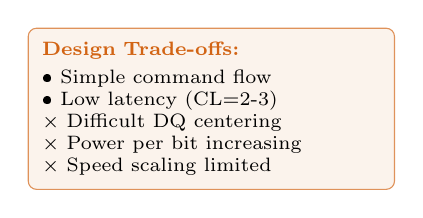
\begin{tikzpicture}[scale=0.85]
        \node[rectangle, rounded corners=3pt, draw=ddr1orange!70, fill=ddr1orange!8,
              text width=4.3cm, align=left, inner sep=5pt, font=\scriptsize] at (0,0)
             {\textbf{\color{ddr1orange}Design Trade-offs:}\\[2pt]
              • Simple command flow\\
              • Low latency (CL=2-3)\\
              $\times$ Difficult DQ centering\\
              $\times$ Power per bit increasing\\
              $\times$ Speed scaling limited};
      \end{tikzpicture}
    \end{column}
  \end{columns}
\end{frame}

% ===================================================================
% SLIDE 7: DDR2 OVERVIEW
% ===================================================================
\begin{frame}{DDR2 (JESD79-2): Architectural Improvements}
  \begin{columns}[T]
    \begin{column}{0.50\textwidth}
      \textbf{Major Enhancements:}
      \begin{itemize}
        \setlength\itemsep{7pt}
        \item \textbf{4:1 Prefetch} → 4 bits per cell per access
        \item \textbf{8 Banks} → double parallelism vs DDR1
        \item \textbf{VDD = 1.8 V} → 28\% lower power
        \item \textbf{ODT On-Die} → controller-driven, no PCB resistors
        \item \textbf{DQS Center-Aligned} → easier capture, no internal centering
        \item Data rates: 400–1066 MT/s
      \end{itemize}
    \end{column}
    \begin{column}{0.48\textwidth}
      \vspace{0.2cm}
      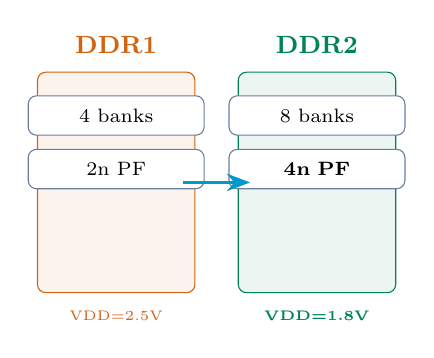
\begin{tikzpicture}[scale=0.85]
        % DDR1 box
        \node[rectangle, rounded corners=3pt, draw=ddr1orange, fill=ddr1orange!8,
              minimum width=2.0cm, minimum height=2.8cm] (d1) at (-1.5, 0) {};
        \node[font=\small\bfseries, color=ddr1orange, above=0.1cm of d1.north] {DDR1};
        \node[sblock] (a1) at (-1.5, 1.0) {4 banks};
        \node[sblock] (p1) at (-1.5, 0.2) {2n PF};
        \node[font=\tiny, color=ddr1orange, below=0.1cm of d1.south] {VDD=2.5V};
        
        % DDR2 box
        \node[rectangle, rounded corners=3pt, draw=ddr2green, fill=ddr2green!8,
              minimum width=2.0cm, minimum height=2.8cm] (d2) at (1.5, 0) {};
        \node[font=\small\bfseries, color=ddr2green, above=0.1cm of d2.north] {DDR2};
        \node[sblock] (a2) at (1.5, 1.0) {8 banks};
        \node[sblock] (p2) at (1.5, 0.2) {\textbf{4n PF}};
        \node[font=\tiny, color=ddr2green, below=0.1cm of d2.south] {\textbf{VDD=1.8V}};
        
        % Arrow
        \draw[-Stealth, very thick, ddracent] (-0.5, 0) -- (0.5, 0);
      \end{tikzpicture}
    \end{column}
  \end{columns}
\end{frame}

% ===================================================================
% SLIDE 8: DDR2 NEW FEATURES
% ===================================================================
\begin{frame}{DDR2: New Features – ODT, Additive Latency, Multi-Bank}
  \begin{columns}[T]
    \begin{column}{0.50\textwidth}
      \textbf{On-Die Termination (ODT):}
      \begin{itemize}
        \setlength\itemsep{5pt}
        \item Resistors built \textbf{inside the DRAM}
        \item Controller enables via \textbf{ODT signal}
        \item Values: 50\,$\Omega$, 75\,$\Omega$, 150\,$\Omega$ (set in EMR)
        \item Reduces reflections → better SI at speed
      \end{itemize}
      
      \vspace{0.3cm}
      \textbf{8 Banks:}
      \begin{itemize}
        \setlength\itemsep{5pt}
        \item Opens more rows in parallel
        \item Better command interleaving
        \item Requires new constraint: \textbf{tFAW} (Four Activate Window)
      \end{itemize}
    \end{column}
    \begin{column}{0.48\textwidth}
      \vspace{0.2cm}
      \textbf{Additive Latency (AL):}
      \vspace{0.15cm}
      
      READ command can be issued early (at ACTIVATE time) → DRAM queues internally.
      
      \vspace{0.3cm}
      \small
      \begin{tabular}{l l}
        \toprule
        \textbf{No AL} & \textbf{With AL=1} \\
        \midrule
        ACT → wait tRCD & ACT (at cycle 0) \\
        READ (at +tRCD) & READ (at cycle 1) \\
        Data at tRCD+CL & Data at AL+CL \\
        & (same absolute time) \\
        \bottomrule
      \end{tabular}
      
      \vspace{0.25cm}
      → Better bus utilization, pipelined commands
    \end{column}
  \end{columns}
\end{frame}

% ===================================================================
% SLIDE 9: DDR2 TIMING CONCEPTS
% ===================================================================
\begin{frame}{DDR2: Timing Concepts – RL, WL, CWL}
  \begin{columns}[T]
    \begin{column}{0.50\textwidth}
      \textbf{Read/Write Latencies:}
      \vspace{0.2cm}
      \renewcommand{\arraystretch}{1.5}
      \small
      \begin{tabular}{l l}
        \toprule
        \textbf{Term} & \textbf{Definition} \\
        \midrule
        \textcolor{ddr2green}{RL (Read Latency)} & AL + CL \\
        \textcolor{ddr2green}{WL (Write Latency)} & AL + CWL \\
        \textcolor{ddr2green}{CWL (CAS Write Latency)} & Separate from CL \\
        tRCD & RAS-to-CAS delay \\
        \bottomrule
      \end{tabular}
      
      \vspace{0.4cm}
      \textbf{Example (DDR2-800):}
      \begin{itemize}
        \setlength\itemsep{6pt}
        \item CL = 5 cycles, AL = 0 or 3
        \item CWL = 5 cycles
        \item RL = 5 (AL=0) or 8 (AL=3)
        \item WL = 5 (AL=0) or 8 (AL=3)
      \end{itemize}
    \end{column}
    \begin{column}{0.48\textwidth}
      \vspace{0.2cm}
      \textbf{Al Effect on Timing:}
      \vspace{0.15cm}
      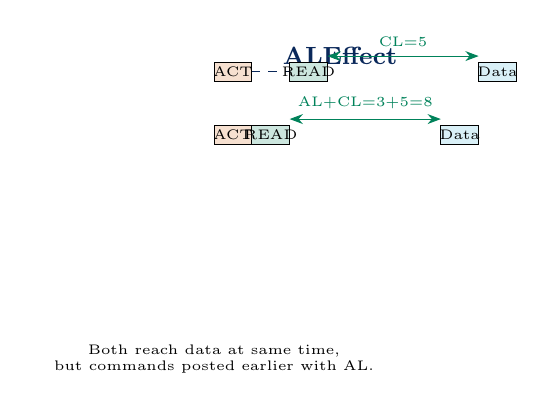
\begin{tikzpicture}[scale=0.8]
        % Case 1: AL=0
        \node[font=\small\bfseries, color=ddrblue] at (2.0, 3.8) {ALEffect};
        \draw[fill=ddr1orange!20] (0, 3.4) rectangle (0.6, 3.7);
        \node[font=\tiny] at (0.3, 3.55) {ACT};
        \draw[dashed, thin, ddrblue] (0.6, 3.55) -- (1.2, 3.55);
        \draw[fill=ddr2green!20] (1.2, 3.4) rectangle (1.8, 3.7);
        \node[font=\tiny] at (1.5, 3.55) {READ};
        \draw[fill=ddracent!15] (4.2, 3.4) rectangle (4.8, 3.7);
        \node[font=\tiny] at (4.5, 3.55) {Data};
        \draw[darrow, ddr2green, thin] (1.8, 3.8) -- (4.2, 3.8)
             node[midway, above, font=\tiny] {CL=5};
        
        % Case 2: AL=3
        \draw[fill=ddr1orange!20] (0, 2.4) rectangle (0.6, 2.7);
        \node[font=\tiny] at (0.3, 2.55) {ACT};
        \draw[fill=ddr2green!20] (0.6, 2.4) rectangle (1.2, 2.7);
        \node[font=\tiny] at (0.9, 2.55) {READ};
        \draw[fill=ddracent!15] (3.6, 2.4) rectangle (4.2, 2.7);
        \node[font=\tiny] at (3.9, 2.55) {Data};
        \draw[darrow, ddr2green, thin] (1.2, 2.8) -- (3.6, 2.8)
             node[midway, above, font=\tiny] {AL+CL=3+5=8};
        
        \node[font=\tiny, below=0.5cm, text width=4.5cm, align=center]
             {Both reach data at same time,\\but commands posted earlier with AL.};
      \end{tikzpicture}
    \end{column}
  \end{columns}
\end{frame}

% ===================================================================
% SLIDE 10: COMPARISON TABLE
% ===================================================================
\begin{frame}{DDR1 vs DDR2: Comprehensive Comparison}
  \centering
  \small
  \renewcommand{\arraystretch}{1.3}
  \vspace{-0.2cm}
  \begin{tabular}{>{\bfseries}p{2.8cm}
                  >{\centering\arraybackslash\color{ddr1orange}\small}p{3.0cm}
                  >{\centering\arraybackslash\color{ddr2green}\small}p{3.0cm}}
    \toprule
    \textbf{Feature} & \textbf{DDR1} & \textbf{DDR2} \\
    \midrule
    Prefetch & 2n & 4n \\
    Banks & 4 & 8 \\
    VDD & 2.5 V & 1.8 V \\
    DQS Alignment & Edge & Center \\
    ODT & External & On-die \\
    Additive Latency & No & Yes (AL) \\
    CWL (Write) & CL–1 & Separate \\
    tFAW & N/A & 4-ACT window \\
    Speed Range & 200–400 & 400–1066 \\
    I/O Standard & SSTL\_2 & SSTL\_18 \\
    OCD Calibration & No & Yes \\
    DFI Version & 1.0 & 2.1 \\
    \bottomrule
  \end{tabular}
\end{frame}

% ===================================================================
% SLIDE 11: KEY TAKEAWAYS
% ===================================================================
\begin{frame}{Key Takeaways}
  \begin{columns}[T]
    \begin{column}{0.48\textwidth}
      \vspace{-0.2cm}
      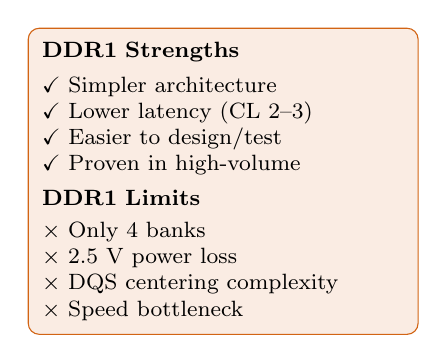
\begin{tikzpicture}[scale=0.85]
        \node[ddr1box=4.8cm, text width=4.6cm, align=left, inner sep=5pt, font=\footnotesize] at (0,0)
             {\textbf{DDR1 Strengths}\\[3pt]
              $\checkmark$ Simpler architecture\\
              $\checkmark$ Lower latency (CL 2–3)\\
              $\checkmark$ Easier to design/test\\
              $\checkmark$ Proven in high-volume\\[3pt]
              \textbf{DDR1 Limits}\\[2pt]
              $\times$ Only 4 banks\\
              $\times$ 2.5 V power loss\\
              $\times$ DQS centering complexity\\
              $\times$ Speed bottleneck};
        \end{tikzpicture}
    \end{column}
    \begin{column}{0.48\textwidth}
      \vspace{-0.2cm}
      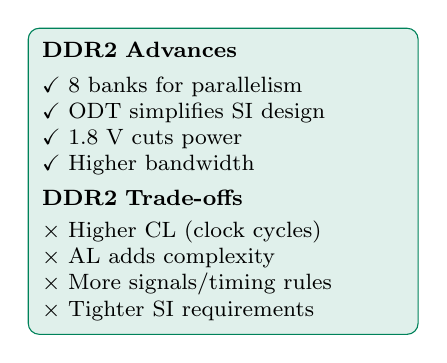
\begin{tikzpicture}[scale=0.85]
        \node[ddr2box=4.8cm, text width=4.6cm, align=left, inner sep=5pt, font=\footnotesize] at (0,0)
             {\textbf{DDR2 Advances}\\[3pt]
              $\checkmark$ 8 banks for parallelism\\
              $\checkmark$ ODT simplifies SI design\\
              $\checkmark$ 1.8 V cuts power\\
              $\checkmark$ Higher bandwidth\\[3pt]
              \textbf{DDR2 Trade-offs}\\[2pt]
              $\times$ Higher CL (clock cycles)\\
              $\times$ AL adds complexity\\
              $\times$ More signals/timing rules\\
              $\times$ Tighter SI requirements};
        \end{tikzpicture}
    \end{column}
  \end{columns}
  
  \vspace{0.4cm}
  \begin{center}
    {\color{ddracent}\rule{0.75\linewidth}{1pt}}\\[0.2cm]
    {\color{ddrblue}\normalsize\bfseries Memory Evolution}\\
    {\small DDR2 trades latency for bandwidth \& efficiency.}
  \end{center}
\end{frame}

% ===================================================================
% SLIDE 12: SUMMARY
% ===================================================================
{
\setbeamercolor{background canvas}{bg=ddrblue}
\begin{frame}[plain]
  \vspace{0.3cm}
  \begin{center}
    {\color{white}\Large\bfseries Summary}
  \end{center}
  
  \vspace{0.5cm}
  \begin{columns}[T]
    \begin{column}{0.48\textwidth}
      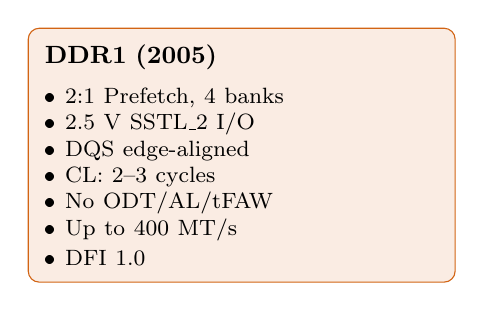
\begin{tikzpicture}[scale=0.95]
        \node[ddr1box=5.2cm, text width=5.0cm, align=left, inner sep=6pt, font=\small] at (0,0)
             {\textbf{\small DDR1 (2005)}\\[5pt]
              {\color{black}\footnotesize
              • 2:1 Prefetch, 4 banks\\
              • 2.5 V SSTL\_2 I/O\\
              • DQS edge-aligned\\
              • CL: 2–3 cycles\\
              • No ODT/AL/tFAW\\
              • Up to 400 MT/s\\
              • DFI 1.0}};
      \end{tikzpicture}
    \end{column}
    \begin{column}{0.48\textwidth}
      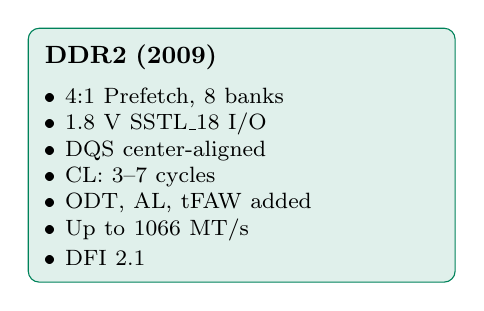
\begin{tikzpicture}[scale=0.95]
        \node[ddr2box=5.2cm, text width=5.0cm, align=left, inner sep=6pt, font=\small] at (0,0)
             {\textbf{\small DDR2 (2009)}\\[5pt]
              {\color{black}\footnotesize
              • 4:1 Prefetch, 8 banks\\
              • 1.8 V SSTL\_18 I/O\\
              • DQS center-aligned\\
              • CL: 3–7 cycles\\
              • ODT, AL, tFAW added\\
              • Up to 1066 MT/s\\
              • DFI 2.1}};
      \end{tikzpicture}
    \end{column}
  \end{columns}
  
  \vspace{0.5cm}
  \begin{center}
    {\color{ddrlite}\footnotesize\itshape
      DDR2: $2.7\times$ bandwidth, 28\% lower power than DDR1\\
      Key: more banks, on-die termination, posted commands}
  \end{center}
\end{frame}
}

\end{document}
